\documentclass[12pt]{article}
\usepackage[a4paper,margin=0.8in]{geometry} % 明確設定四邊
\usepackage{fontspec}
\usepackage{xeCJK}
\usepackage{titling} % 預設標題下移0.6in
\usepackage{amsmath} % 數學方程式
\usepackage{graphicx} %圖片
\usepackage{float} % 在導言區 ,讓圖片強制插在原地
\usepackage{xcolor} %字體加入顏色
\usepackage{hyperref} % 引入網址
\usepackage{physics} % 物理符號
\usepackage{wrapfig} % 文字環繞圖片
\setmainfont{Times New Roman}
\setCJKmainfont{Kaiti TC}

\setlength{\droptitle}{-1in} % 上移標題0.6in
\title{Assignment 1}
\author{學號:114233515陳芃仲\\}
\begin{document} 
\maketitle 


\noindent 利用有限體積法$FVM$求解二維穩態擴散對流方程:\\
\noindent 推導一般形式下的擴散對流方程:
\noindent 無外源項的純擴散方程,構成一laplace方程:
\begin{equation}
    k\nabla^2 T= 0\\
\end{equation}
\noindent 一般令擴散係數$k$為均勻場。
\noindent 寫成分量形式則有:
\begin{equation}
    \begin{split}
        \frac{\partial }{\partial x}(k \frac{\partial T }{\partial x}) + \frac{\partial }{\partial y}(k \frac{\partial T }{\partial y}) = 0
    \end{split}
\end{equation}
\noindent 本方程不考慮外源項,因此為lapalce方程,否則為possion方程。\\
\noindent 邊界條件:
\begin{equation}
    \begin{split}
        T(x, 0) &= T_{x,0} = 0\\
        T(x, L) &= T_{x,L}= 1\\
        T(0, y) &= T_{0,y} = 0\\
        T(L, y) &= T_{L,y} = 0
    \end{split}
\end{equation}
\noindent 其中$T_{1L}$為上邊界溫度,$T_{0L}$為左邊界溫度,$T_{0R}$為右邊界溫度$T_{1L}$為上邊界溫度,$T_{0L}$為左邊界溫度。
\noindent 由於本方程為二維穩態擴散對流方程,因此對時間無關,且對於二維空間$(x,y)$,對於每個空間點$(x,y)$,其溫度$T(x,y)$均為常數。\\
\noindent 本邊界採用link-wise邊界,且個別邊界條件為Dirichlet邊界條件。需要注意的是:在對應非齊性邊界條件的邊界點上,離散方程需要將固定溫度輸入作為外源項。\\
\begin{wrapfigure}{r}{0.3\textwidth}%圖片外邊界佔整個文本寬度
    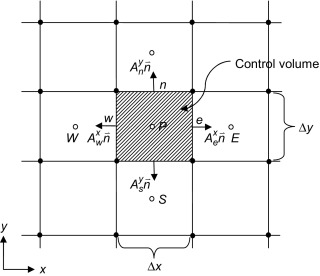
\includegraphics[width=0.3\textwidth]{1.jpg}
\end{wrapfigure}
\noindent (一)、第一步,如右圖所示,把整個二維空間拆成$(N_x,N_y)$個格子,且由於採用link-wise邊界,computatial node分佈於格點中心,且computatioal boundary與physical boundary總是距離半格子長度。
圖中,陰影區域為計算點p的控制體積(control volume),控制體積介面w,e之距離為$\Delta x$,控制體積介面n,s之距離為$\Delta y$。由於網格化分為均勻網格,故$\Delta x = \Delta y $。且計算點p與相鄰各個計算點的距離均為
$\Delta x$ 。因此, 離散化邊界範圍:$i = (0 : N_x) , j = (0 : N_y)$

若p點位置為$(i,j)$,則其鄰居點分別為:
\begin{equation}
    \begin{split}
        p_{left} &= (i-\frac{1}{2},j)\\
        p_{right} &= (i+\frac{1}{2},j)\\
        p_{up} &= (i,j+\frac{1}{2})\\
        p_{down} &= (i,j-\frac{1}{2})
    \end{split}
\end{equation}
\noindent (二)、構造擴散方程的離散化格式:
\noindent 由無外源的擴散方程積分形式可得:
\begin{align}
    \int_{\Delta V} dV\vec{\nabla} \cdot (k \vec{\nabla} T) =   \int_{\Delta V} dV \frac{\partial }{\partial x}(k \frac{\partial T }{\partial x}) + \int_{\Delta V} dV \frac{\partial }{\partial y}(k \frac{\partial T }{\partial y}) = 0
\end{align}
\noindent 其中,$dV = dx\cdot dy$ 。積分區域為單格網格空間。
\noindent 被積分函數事實上為散度項之分量形式,型如 $\vec{\nabla} \cdot (k \vec{\nabla} T)$。利用高斯散度定理可化為:(面積分方向為外法線方向)
\begin{align}
    &\oint_{\partial (\Delta V)} d\vec{a} \cdot (k \vec{\nabla} T) = 0\\
    &-\int_{left} dy (k \frac{\partial T }{\partial x}) +\int_{right} dy (k \frac{\partial T }{\partial x})
    +\int_{up} dx (k \frac{\partial T }{\partial y}) - \int_{down} dx (k \frac{\partial T }{\partial y})
    = 0 
\end{align}
\noindent 由於$dx ,dy \rightarrow 0 $ 時,可將上式寫為:
\begin{align}
-dy ( \frac{\partial T }{\partial x})(x,y) +dy (k \frac{\partial T }{\partial x})(x+\Delta x,y)
+dx (k \frac{\partial T }{\partial y})(x,y+\Delta y) -dx (k \frac{\partial T }{\partial y})(x,y)
= 0\\
dx\cdot dy\frac{\partial T }{\partial x} (k \frac{\partial T }{\partial x})(x,y) +
+dx\cdot dy\frac{\partial T }{\partial y} (k \frac{\partial T }{\partial y})(x,y) 
= 0
\end{align}
\noindent 而由於$\Delta x \neq dx ,\Delta y \neq dy $,這裡需要做兩次一階精度近似:\\
\noindent 對於$$-\int_{left} dy (k \frac{\partial T }{\partial x}) +\int_{right} dy (k \frac{\partial T }{\partial x})
    +\int_{up} dx (k \frac{\partial T }{\partial y}) - \int_{down} dx (k \frac{\partial T }{\partial y})
    $$近似為:$$-\Delta y ( k\frac{\partial T }{\partial x})(x,y) +\Delta y (k \frac{\partial T }{\partial x})(x+\Delta x,y)
+\Delta x (k \frac{\partial T }{\partial y})(x,y+\Delta y) -\Delta x (k \frac{\partial T }{\partial y})(x,y)
$$
\noindent 若$(x,y)$為有限體積中心點$p\quad (i,j)$,對有限體積之邊界點:$$n\_point = (i,j+1), s\_point = (i,j-1), e\_point = (i+1,j), w\_point = (i-1,j)$$
進行一階近似後,則有:
\begin{align}
    \Delta y (k \frac{\partial T }{\partial x})_{(i+\frac{1}{2},j)}-\Delta y ( k\frac{\partial T }{\partial x})_{(i-\frac{1}{2},j)} 
    +\Delta x (k \frac{\partial T }{\partial y})_{(i,j+\frac{1}{2})} -\Delta x (k \frac{\partial T }{\partial y})_{(i,j-\frac{1}{2})}
    = 0
\end{align}
\noindent 引入($w$($o$($f$雙變數函數)的($x$變數一階偏導數))的(二階精度中心差分)):
\begin{align}
    \frac{f(x+\Delta x,y)-f(x-\Delta x,y)}{2\cdot \Delta x} = \left.\frac{\partial f }{\partial x} \right|_{(x,y)}+\O(\Delta x^{2})
\end{align}
\noindent 再對左點,下點,上點,右點作二階精度中心差分$(dif\quad instance = \frac{\Delta x}{2})$,有:(因此,精度在空間中為二階精度)
\begin{equation}
    \begin{split}
 &\Delta y (  \cdot k \frac{T_{i+1,j}-T_{i,j}}{\Delta x})- \Delta y (  \cdot k \frac{T_{i,j}-T_{i-1,j}}{\Delta x})\\
 &+ \Delta x (  \cdot k \frac{T_{i,j+1}-T_{i,j}}{\Delta y})- \Delta x (  \cdot k \frac{T_{i,j}-T_{i,j-1}}{\Delta y}) = 0\\
\end{split}
\end{equation}
\noindent 上式即為均勻網格下(網格正交分佈且$\Delta x = \Delta y$)的二維穩態擴散方程的空間二階精度中心蘇離散格式。整理上式有:\\
\begin{equation}
    \begin{split}
 &\Delta y ( \frac{T_{i+1,j}}{\Delta x})+ \Delta y ( \frac{T_{i-1,j}}{\Delta x}) + \Delta x ( \frac{T_{i,j+1}}{\Delta y})+ \Delta x ( \frac{T_{i,j-1}}{\Delta y})\\
 &= (( \frac{\Delta y}{\Delta x})+ ( \frac{\Delta y }{\Delta x}) + ( \frac{\Delta x}{\Delta y})+ ( \frac{\Delta x}{\Delta y}))\cdot T_{i,j}\\
\end{split}
\end{equation}
\noindent 更簡潔一點,可以寫為:
\begin{equation}
    \begin{split}
 &(\frac{\Delta y }{\Delta x})\cdot (T_{right} + T_{left})+  \frac{\Delta x}{\Delta y}\cdot (T_{up} + T_{bottom})\\
 &= 2(( \frac{\Delta y}{\Delta x})+( \frac{\Delta x}{\Delta y}))\cdot T_{p}\\
\end{split}
\end{equation}
但是,上條件為簡化版,廣義來説:近似規則為$(1)$對外法線方向熱流密度$\frac{\partial T}{\partial n} =\vec{n}\cdot  \vec{q}$取二階精度中心差分,$(2)$對邊界擴散係數(考慮非均勻場)取平均值,則得到二維穩態純擴散方程的空間二階精度中心離散格式,以下說明\\
\noindent 若網格在$n\_point,s\_point,e\_point,w\_point $處的外法向熱流密度($\frac{\partial T}{\partial n} =\vec{n}\cdot  \vec{q})$,非均勻擴散係數($k$),面積($A$)分別為:\\
\noindent $$\frac{\partial T}{\partial n}_{w} = \frac{T_{i,j}-T_{i-1,j}}{\Delta x_{pW}}, \frac{\partial T}{\partial n}_{e} = \frac{T_{i+1,j}-T_{i,j}}{\Delta x_{Ep}}, \frac{\partial T}{\partial n}_{s} = \frac{T_{i,j}-T_{i,j-1}}{\Delta y_{pS}}, \frac{\partial T}{\partial n}_{n} = \frac{T_{i,j+1}-T_{i,j}}{\Delta y_{Np}}$$\\
\noindent $$k_{w} = \frac{k_{i-1,j}+k_{i,j}}{2}, k_{e} = \frac{k_{i,j}+k_{i+1,j}}{2}, k_{s}  = \frac{k_{i,j}+k_{i,j-1}}{2}, k_{n} = \frac{k_{i,j}+k_{i,j+1}}{2}$$\\
\noindent $$A_{w} = A_{i-\frac{1}{2},j}, A_{e} = A_{i+\frac{1}{2},j}, A_{s}  = A_{i,j-\frac{1}{2}}, A_{n} = A_{i,j+\frac{1}{2}}$$\\
\noindent 且 $(W,E,S,N)\_computational\_point$至 中心點$p\quad (i,j)$的距離分別為:$$\Delta x_{pW} , \Delta x_{Ep} , \Delta y_{pS} , \Delta y_{Np}$$\\
\noindent 則二維穩態擴散方程的空間二階精度中心離散格式:
\begin{equation}
    \begin{split}
 &A_{e}   \cdot (\frac{k_{i+1,j}+k_{i,j}}{2} \frac{T_{i+1,j}-T_{i,j}}{\Delta x_{Ep}})- A_{w}   \cdot (\frac{k_{i,j}+k_{i-1,j}}{2} \frac{T_{i,j}-T_{i-1,j}}{\Delta x_{pW}})\\
 &+ A_{n}   \cdot (\frac{k_{i,j+1}+k_{i,j}}{2} \frac{T_{i,j+1}-T_{i,j}}{\Delta y_{Np}})- A_{s}   \cdot (\frac{k_{i,j}+k_{i,j-1}}{2} \frac{T_{i,j}-T_{i,j-1}}{\Delta y_{pS}}) = 0\\
\end{split}
\end{equation}
形成:
\begin{equation}
    \begin{split}
        a_{p}T_{p} &= a_{W}T_{W} + a_{E}T_{E} +  a_{S}T_{S} + a_{N}T_{N}  \\
    \end{split}
\end{equation}
\noindent 其中,
\begin{equation}
    \begin{split}
        &T_{p} = T_{i,j} , a_{p} = a_{W} + a_{E} + a_{S} + a_{N}\\
        &T_{W} = T_{i-1,j}, a_{W} = A_{w}\frac{k_{i,j}+k_{i-1,j}}{2 \Delta x_{pW}} \\
        &T_{E} = T_{i+1,j}, a_{E} = A_{e}\frac{k_{i+1,j}+k_{i,j}}{2\Delta x_{Ep}}\\
        &T_{S} = T_{i,j-1}, a_{S} = A_{s}\frac{k_{i,j}+k_{i,j-1}}{2\Delta y_{pS}}\\
        &T_{N} = T_{i,j+1}, a_{N} = A_{n}\frac{k_{i,j+1}+k_{i,j}}{2\Delta y_{Np}}\\
    \end{split}
\end{equation}
\noindent ,上式亦為2D steady state diffusion eqaution 的二階精度中心離散格式。\\
\vspace{0.7em}\\
\noindent (三)、邊界處理\\
\noindent 此邊界採用:Link-Wise分佈,邊界計算點與物理邊界相距半個格子長。
\noindent 針對非齊性邊條件,處理邊界點應該滿足的離散化方程:
\noindent 由於$T(x,L) = T_{i,Ny+\frac{1}{2}}= 1.0$ ,則對於邊界上的computational node$(i,Ny)$,其離散化方程
\noindent 由(12)做修改。(先寫出邊界點的離散方程,再帶入邊界條件)\\
\noindent 處理方式:\\
\noindent ($w$($W$($L$左計算格點)的(西邊界點))的(體熱流密度))取一階前項差分(中心-本位):\\
\noindent (($w$($W$($L$左計算格點)的(西邊界點))的(體熱流密度))的(一階精度前項差分)):$$ q_{x(-\delta_{W},j)}=\frac{T_{0,j} - T_{-\delta_{W},j} }{\Delta x_{pw}} ,q_{x(-\frac{1}{2},j)}=\frac{T_{0,j} - T_{-\frac{1}{2},j}}{\frac{\Delta x}{2}} $$
\noindent ($e$($E$($R$右計算格點)的(東邊界點))的(體熱流密度))取一階後項差分(本位-中心):\\
\noindent (($e$($E$($R$右計算格點)的(東邊界點))的(體熱流密度))的(一階精度後項差分)):$$ q_{x(Nx+\delta_{E},j)}=\frac{T_{Nx+\delta_{E},j} - T_{Nx,j}}{\Delta x_{ep}}, q_{x(Nx+\frac{1}{2},j)}=\frac{T_{Nx+\frac{1}{2},j} - T_{Nx,j}}{\frac{\Delta x}{2}} $$
\noindent ($s$($S$($B$下計算格點)的(南邊界點))的(體熱流密度))取一階前項差分:(中心-本位)\\
\noindent (($s$($S$($B$下計算格點)的(南邊界點))的(體熱流密度))的(一階精度前項差分)):$$ q_{x(i,-\delta_{S})}=\frac{ T_{i,0} - T_{i,-\delta_{S}}}{\Delta y_{ps}} , q_{x(i,-\frac{1}{2})}=\frac{T_{i,0} - T_{i,-\frac{1}{2}}}{\frac{\Delta y}{2}} $$
\noindent ($n$($N$($U$上計算格點)的(北邊界點))的(體熱流密度))取一階後項差分(本位-中心):\\
\noindent (($n$($N$($U$上計算格點)的(北邊界點))的(體熱流密度))的(一階精度後項差分)):$$ q_{x(i,Ny+\delta_{N})}=\frac{T_{i,Ny+\delta_{N}} - T_{i,Ny}}{\Delta y_{np}} , q_{x(i,Ny+\frac{1}{2})}=\frac{T_{i,Ny+\frac{1}{2}} - T_{i,Ny}}{\frac{\Delta y}{2}} $$
\noindent 此題上邊界計算點離散化方程:(均勻正交網格、邊場條件特殊)
\begin{equation}
    \begin{split}
 &\Delta y  \cdot  (k \frac{T_{i+1,Ny}-T_{i,Ny}}{\Delta x})- \Delta y \cdot (k \frac{T_{i,Ny}-T_{i-1,Ny}}{\Delta x})\\
 &+0 - \Delta x \cdot (k \frac{T_{i,Ny}-T_{i,Ny-1}}{\Delta y})+ {\color{red}\Delta x\cdot( k \frac{T_{i,Ny+\frac{1}{2}}-T_{i,Ny}}{\frac{\Delta y}{2}})} = 0\\
\end{split}
\end{equation}
\noindent 壁面上的擴散係數$k_{i,Ny+\frac{1}{2}}$仍取用p點上的擴散係數$k_{i,Ny}$。一般來說,內點上的擴散係數$k_{i,j+\frac{1}{2}}$採用迎風離散:$\frac{k_{N}+k_{p}}{2}$\\
\noindent 上式可化為:(各項係數之分子為該面闊散係數$k$乘上該面積分空間$A$,分母為差分距離)
\begin{equation}
    \begin{split}
 &\frac{\Delta y   \cdot k}{\Delta x}T_{i-1,Ny}+  \frac{\Delta y \cdot k}{\Delta x}T_{i+1,Ny}+
  \frac{\Delta x   \cdot k }{\Delta y}T_{i,Ny-1}+0  + {\color{red}\frac{\Delta x\cdot k }{\frac{\Delta y}{2}}T_{i,Ny+\frac{1}{2}}}\\
=&\frac{\Delta y   \cdot k }{\Delta x}T_{i,Ny} + \frac{\Delta y \cdot k }{\Delta x}T_{i,Ny} + 0 + \frac{\Delta x \cdot k }{\Delta y}T_{i,Ny} + {\color{red}\frac{\Delta x\cdot k }{\frac{\Delta y}{2}}T_{i,Ny}} \\
\end{split}
\end{equation}
\begin{equation}
    \begin{split}
 &\frac{\Delta y   \cdot k}{\Delta x}T_{i-1,Ny}+  \frac{\Delta y \cdot k}{\Delta x}T_{i+1,Ny}+
 \frac{\Delta x   \cdot k }{\Delta y}T_{i,Ny-1} + 0 + {\color{red}\frac{\Delta x\cdot k }{\frac{\Delta y}{2}}T_{i,Ny+\frac{1}{2}}}\\
=&\left[\frac{\Delta y   \cdot k }{\Delta x}+ \frac{\Delta y \cdot k }{\Delta x} + 0 + \frac{\Delta x   \cdot k }{\Delta y} - {\color{red}(-\frac{\Delta x\cdot k }{\frac{\Delta y}{2}}Q)} \right]T_{i,Ny}\\
\end{split}
\end{equation}
\newpage
\noindent 通用的$up\,boundary\,computational\,node (i,Ny)$所滿足的離散化方程為:\\
\begin{equation}
    \begin{split}
 &A_{e}  \cdot  (\frac{k_{i+1,Ny}+k_{i,Ny}}{2} \frac{T_{i+1,Ny}-T_{i,Ny}}{\Delta x_{Ep}})- A_{w}  \cdot  (\frac{k_{i,Ny}+k_{i-1,Ny}}{2} \frac{T_{i,Ny}-T_{i-1,Ny}}{\Delta x_{pW}})\\
 &+0- A_{s}  \cdot(  \frac{k_{i,Ny}+k_{i,Ny-1}}{2} \frac{T_{i,Ny}-T_{i,Ny-1}}{\Delta y_{pS}}) + {\color{red}A_{n}(k_{i,Ny}\frac{T_{i,Ny+\frac{1}{2}}-T_{i,Ny}}{\Delta y_{np}})}= 0\\
\end{split}
\end{equation}
\noindent 將非齊性邊界條件的影響放到外源項中,形成:
\begin{equation}
    \begin{split}
        &(a_{up,W}+ a_{up,E}+ a_{up,S}+ a_{up,N}-S_{up,p})T_{up,p} \\
        &= a_{up,W}T_{up,W} + a_{up,E}T_{up,E} \\
        &+  a_{up,S}T_{up,S} + a_{up,N}T_{up,N} \\
        & + S_{up,u} \\
    \end{split}
\end{equation}
\noindent 其中,
\begin{equation}
    \begin{split}
        T_{up,p} &= T_{i,Ny} \\
        S_{up,p} &= -A_{n}\frac{k_{i,Ny}}{\Delta y_{np}}\\
        T_{up,W} &= T_{i-1,Ny}, a_{W} = A_{w}\frac{\frac{k_{i,Ny}+k_{i-1,Ny}}{2}}{ \Delta x_{pW}} \\
        T_{up,E} &= T_{i+1,Ny}, a_{E} = A_{e}\frac{\frac{k_{i+1,Ny}+k_{i,Ny}}{2}}{\Delta x_{Ep}}\\
        T_{up,S} &= T_{i,Ny-1}, a_{S} = A_{s}\frac{\frac{k_{i,Ny}+k_{i,Ny-1}}{2}}{\Delta y_{pS}}\\
        T_{up,N} &= 0 ,a_{N} = 0 \\
        S_{up,u} &=A_{n}\frac{k_{i,Ny}}{\Delta y_{np}}\cdot T_{i,Ny+\frac{1}{2}}\\
    \end{split}
\end{equation}
\noindent 此題左邊界計算點離散化方程:(均勻正交網格、邊場條件特殊)\\
\begin{equation}
    \begin{split}
 & 0 +  \frac{\Delta y \cdot k}{\Delta x}T_{1,j}+
 \frac{\Delta x \cdot k}{\Delta y}T_{0,j-1}+ \frac{\Delta x   \cdot k }{\Delta y}T_{0,j+1} + {\color{red}\frac{\Delta y\cdot k }{\frac{\Delta x}{2}}T_{-\frac{1}{2},j}}\\
=&\left[0+ \frac{\Delta y   \cdot k }{\Delta x}+ \frac{\Delta x \cdot k }{\Delta y} + \frac{\Delta x   \cdot k }{\Delta y} -{\color{red} ( -  \frac{\Delta y\cdot k }{\frac{\Delta x}{2}})}\right]T_{i,Ny}  \\
\end{split}
\end{equation}
\noindent 通用的$left\,boundary\,computational\,node (i,Ny)$所滿足的離散化方程為:\\
\begin{equation}
\begin{split}
    &(a_{left,W}+a_{left,E}+a_{left,S}+a_{left,N}-S_{left,p})T_{left,p}\\
    &= a_{left,W}T_{left,W} + a_{left,E}T_{left,E} \\
    &+a_{left,S}T_{left,S} + a_{left,N}T_{left,N}\\
    &+S_{left,u}\\
\end{split}
\end{equation}
\noindent 其中,
\begin{equation}
    \begin{split}
        &T_{left,p} = T_{0,j} \\
        &S_{left,p} = -A_{w}\frac{k_{0,j}}{\Delta x_{pw}}\\
        &T_{left,W} = 0 , a_{W} = 0\\
        &T_{left,E} = T_{1,j}, a_{E} = A_{e}\frac{\frac{k_{1,j}+k_{0,j}}{2}}{\Delta x_{Ep}}\\
        &T_{left,S} = T_{0,j-1}, a_{S} = A_{s}\frac{\frac{k_{0,j-1}+k_{0,j}}{2}}{\Delta y_{pS}}\\
        &T_{left,N} = T_{0,j+1} ,a_{N} = A_{n}\frac{\frac{k_{0,j+1}+k_{0,j}}{2}}{\Delta y_{Np}}\\
        &S_{left,u} =A_{w}\frac{k_{0,j}}{\Delta x_{pw}}\cdot T_{-\frac{1}{2},j}\\
    \end{split}
\end{equation}
\noindent 同理,
\noindent 此題右邊界計算點離散化方程:(均勻正交網格、邊場條件特殊)\\
\begin{equation}
    \begin{split}
 &\frac{\Delta y   \cdot k}{\Delta x}T_{Nx-1,j}+0+
 \frac{\Delta x   \cdot k }{\Delta y}T_{Nx,j-1}+ \frac{\Delta x   \cdot k }{\Delta y}T_{Nx,j+1} + {\color{red}\frac{\Delta y\cdot k }{\frac{\Delta x}{2}}T_{Nx+\frac{1}{2},j}}\\
=&\left[\frac{\Delta y   \cdot k }{\Delta x}+ 0 + \frac{\Delta x \cdot k }{\Delta y} +\frac{\Delta x   \cdot k }{\Delta y}- {\color{red}(-\frac{\Delta y\cdot k }{\frac{\Delta x}{2}})} \right]T_{Nx,j} \\
\end{split}
\end{equation}
\noindent 通用的$right\,boundary\,computational\,node (i,Ny)$的離散化方程為:\\
\begin{equation}
\begin{split}
    &(a_{right,W}+a_{right,E}+a_{right,S}+a_{right,N}-S_{right,p})T_{right,p}\\
    &= a_{right,W}T_{right,W} + a_{right,E}T_{right,E} \\
    & +  a_{right,S}T_{right,S} + a_{right,N}T_{right,N}\\
    &+ S_{right,u}\\
\end{split}
\end{equation}
\noindent 其中,
\begin{equation}
    \begin{split}
        T_{right,p} &= T_{Nx,j} \\
        S_{right,p} &= -A_{e}\frac{k_{Nx,j}}{\Delta x_{ep}}\\
        T_{right,W} &= T_{Nx-1,j}, a_{W} = A_{w}\frac{\frac{k_{Nx,j}+k_{Nx-1,j}}{2}}{\Delta x_{pW}}\\
        T_{right,E} &= 0 , a_{E} = 0\\
        T_{right,S} &= T_{Nx,j-1}, a_{S} = A_{s}\frac{\frac{k_{Nx,j-1}+k_{Nx,j}}{2}}{\Delta y_{pS}}\\
        T_{right,N} &= T_{Nx,j+1} ,a_{N} = A_{n}\frac{\frac{k_{Nx,j+1}+k_{Nx,j}}{2}}{\Delta y_{Np}}\\
        S_{right,u} &=A_{w}\frac{k_{Nx,j}}{\Delta x_{ep}}\cdot T_{Nx+\frac{1}{2},j}\\
    \end{split}
\end{equation}
\noindent 此題下邊界計算點離散化方程:(均勻正交網格、邊場條件特殊)\\
\begin{equation}
    \begin{split}
 &\frac{\Delta y   \cdot k}{\Delta x}T_{i-1,0}+  \frac{\Delta y \cdot k}{\Delta x}T_{i+1,0}+
 0 + \frac{\Delta x \cdot k}{\Delta y}T_{i,1} + {\color{red}\frac{\Delta x\cdot k }{\frac{\Delta y}{2}}T_{i,-\frac{1}{2}}}\\
=&\left[\frac{\Delta y   \cdot k }{\Delta x}+ \frac{\Delta y \cdot k }{\Delta x} + 0 + \frac{\Delta x   \cdot k }{\Delta y}- {\color{red}(-\frac{\Delta x\cdot k }{\frac{\Delta y}{2}})} \right]T_{i,0} \\
\end{split}
\end{equation}
\noindent 通用的$bottom\,boundary\,computational\,node (i,Ny)$的離散化方程為:\\
\begin{equation}
\begin{split}
    &(a_{bottom,W}+a_{bottom,E}+a_{bottom,S}+a_{bottom,N}-S_{bottom,p})T_{bottom,p}\\
    &= a_{bottom,W}T_{bottom,W} + a_{bottom,E}T_{bottom,E} \\
    & +  a_{bottom,S}T_{bottom,S} + a_{bottom,N}T_{bottom,N} \\
    & + S_{bottom,u}
\end{split}
\end{equation}
\noindent 其中,
\begin{equation}
    \begin{split}
        &T_{bottom,p} = T_{i,0} \\
        &S_{bottom,p} = -A_{s}\frac{k_{i,0}}{\Delta y_{ps}}\\
        &T_{bottom,W} = T_{i-1,0}, a_{W} = A_{w}\frac{\frac{k_{i,0}+k_{i-1,0}}{2}}{\Delta x_{pW}}\\
        &T_{bottom,E} = T_{i+1,0} , a_{E} = A_{e}\frac{\frac{k_{i+1,0}+k_{i,0}}{2}}{\Delta x_{Ep}}\\
        &T_{bottom,S} = 0, a_{S} =0\\
        &T_{bottom,N} = T_{i,1} ,a_{N} = A_{n}\frac{\frac{k_{i,1}+k_{i,0}}{2}}{\Delta y_{Np}}\\
        &S_{bottom,u} =A_{s}\frac{k_{i,0}}{\Delta y_{ps}}\cdot T_{i,-\frac{1}{2}}\\
    \end{split}
\end{equation}
上述即為二維穩態擴散方程的二階精度中心離散格式的邊界處理。

\end{document}
